\subsection{Hardware} \label{sec:proposed-hardware}

While keeping a careful consideration of characteristics between options and maintaining the requirements in focus, hardware parts were chosen to build each section of the demonstrator.

After some careful consideration and planning, we decided to focus our system on utilizing only one of the supported RTE networks.
After studying current implementations of several RTE network master nodes we concluded EtherCAT \cite{protocol:ethercat} would provide us with more flexibility across almost all fields.
Taking into account their characteristics and features, especially the cyclic communication timings, we decided to use EtherCAT as our RTE network of choice.

\subsubsection{Master node}

Taking into account the two operation modes the demonstrator should have, we extrapolated that the master node must be able to perform numeric calculations and serve as an EtherCAT master device.
As the EtherCAT master implementation can be done using a generic Ethernet MAC interface card (refer to \autoref{subsubsec:master_devices} for an explanation), everything the master node requires in term of hardware is a computational platform (computer, microcontroller, etc.) with access to a generic Ethernet MAC interface card.

As of today, most education facilities provide students with access to desktop computers.
For many years now, motherboard vendors have integrated Ethernet MAC interface cards into the motherboards themselves, as it has become the de facto standard for Internet connectivity in desktop computers.

As such, we decided to implement the master device in a desktop computer in order to minimize costs and leverage the computational power modern computer systems possess.
Regardless, our slave device solution includes hardware support for running either slave or master nodes for EtherCAT and other RTE networks, so it is also possible to implement the master node on a Raspberry Pi.

\subsubsection{Slave node} \label{subsubsec:slave_hdw}

On the other hand, the slave node's hardware was harder to choose.
In order to implement the desired EtherCAT slave (see \autoref{subsubsec:slave_devices}), one must be aware when choosing a computational platform to check the availability of a compatible EtherCAT Slave Controller (ESC) board and, simultaneously, the support for motor and encoder interfaces.

After some research, two options presented themselves as possible platforms for the slave device: an Arduino UNO or a Raspberry Pi.
ESC boards exist for both these platforms, as well as good support in terms of `shield boards' for motor interfaces.
In the end, we decided to go with a solution based on a Raspberry Pi, as it provides a more robust and versatile computing platform, especially considering the local control configuration, where position/velocity control algorithms will need to be executed on this platform.

The ESC chosen for the Raspberry Pi was the Hilscher's \emph{netHAT 52-RTE} board \cite{hdw:nethat-52rte}.
\autoref{fig:nethat-52-rte} shows the board used on the system.
This board supports communication with three real-time Ethernet protocols (PROFINET, EtherNet/IP or EtherCAT), chosen with a simple firmware loading procedure.
It complies with the Hardware Attached on Top (HAT) specification for the Raspberry Pi \cite{technology:hats} and uses the \emph{SPI0} interface to communicate with it.
The board also includes the respective Electronic Data Sheet (EDS) files to be imported by the EtherCAT master.
These are used to identify the characteristics, functionality and addresses of slave devices expected to be present on the network.

\begin{figure}[t]
	\centering
	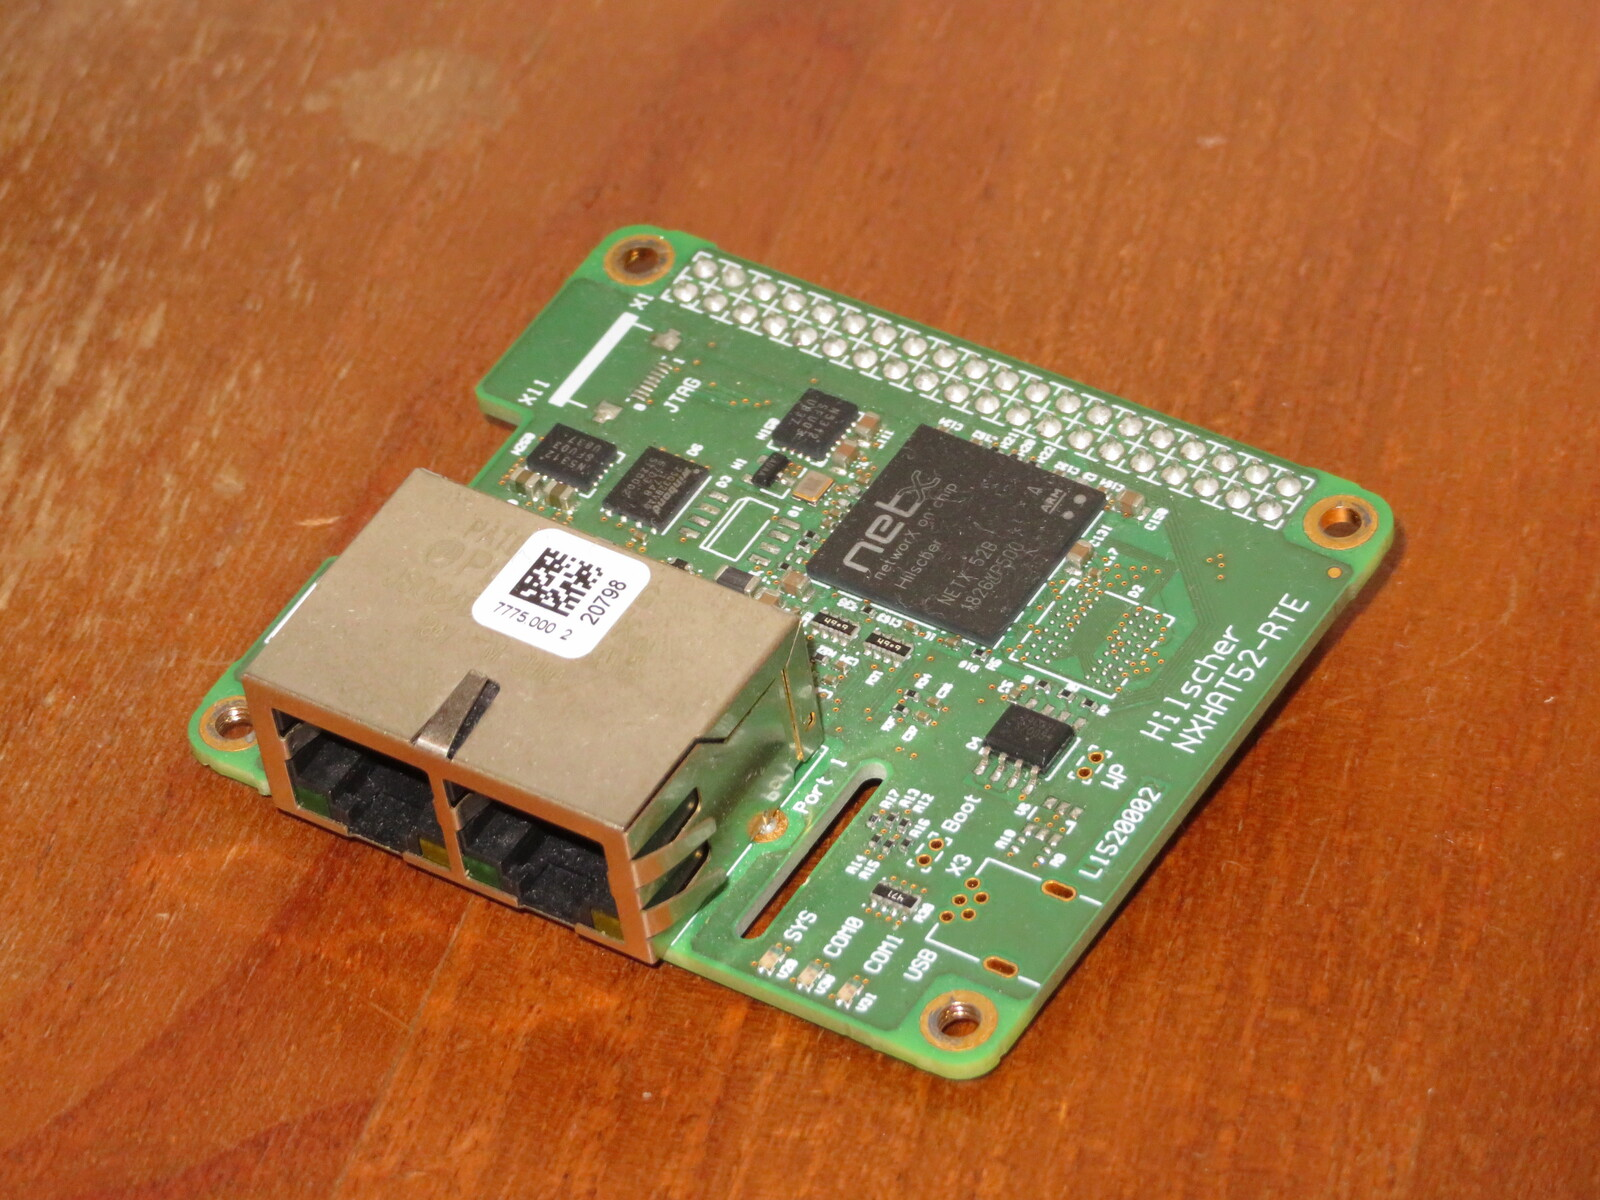
\includegraphics[width=0.8\textwidth]{nethat_52rte.JPG}
	\caption{Hilscher's netHAT 52-RTE board}
	\label{fig:nethat-52-rte}
\end{figure}

% Motor choice
As previously expressed, we intend to make the slave device mimic, to a certain degree, a servo motor drive.
For this two hardware components are fundamental: a motor and a position or velocity feedback mechanism.
As we intend to support position control, we will focus on position feedback products, as velocity can be extrapolated from the sequence of position points.
The most simple and widely used position feedback mechanism is the incremental quadrature encoder, so we'll focus our research efforts into motors that support it.
The most appropriate products we found, keeping in mind the low-cost requirement, are the Pololu's micro metal gearmotor with extended motor shaft \cite{product:pololu-micrometal-gearmotor} paired with the brand's magnetic encoder kit \cite{product:pololu-encoder-kit}.
As this is a DC motor, it's power output can be indirectly controlled if fed with a PWM electrical signal, varying this signal's duty-cycle. % TODO: cite something with explanaition on PWM

With the intention to include a dedicated board to drive the motor, we included the DFRobot's DFR0592 \cite {hdw:dfr0592} board onto the design.
This board also complies with the HAT specification and communicates with the Raspberry Pi via the Inter-Integrated Circuit (I\textsuperscript{2}C or I2C) interface.
It provides interface with two DC motors and two incremental encoders, all managed by an STMicroelectronics's STM32 chip.
The motor interface also includes the necessary DC-motor driver chip, allowing direct connection of the motor's terminals and power supply to the board itself.

Initially we planed on using this board's incremental encoder interface to also relieve the Raspberry Pi from such task but, as our preliminary tests concluded, it only exports the Revolutions Per Minute (RPM) value extrapolated from the encoder's pulse count and not the pulse count itself.
Furthermore, this RPM value is only updated once every 100ms, which is to large of a period for motion control.
To overcome this limitation, we decided to connect the encoder signals directly on the Raspberry's GPIO pins and create a software module to handle them.
This way we will be able to separate the logic that decodes the pulse signals and the position/velocity tracking, allowing us to configure the update period for the latter.

The end result of this process can be seen on \autoref{fig:slave_architecture} (page \pageref{fig:slave_architecture}), which represents the final architecture of the slave device developed throughout this project's lifetime. \footnote{NOTE: Again, just a placeholder image}

\begin{figure}[t]
	\centering
	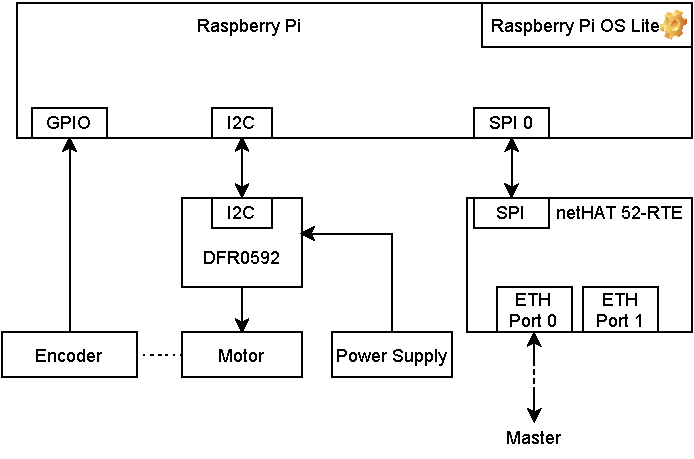
\includegraphics[trim={2cm 12cm 2.5cm 2.5cm},width=0.8\textwidth,clip]{slave_architecture.pdf}
	\caption{Graphical representation of the slave architecture}
	\label{fig:slave_architecture}
\end{figure}
